\section{Architecture}

 \begin{figure}[h]
 \centering
 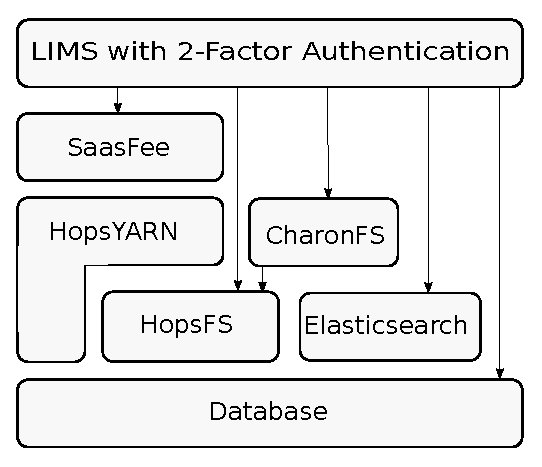
\includegraphics[scale=0.75]{./imgs/stack.eps}
 % stack.eps: 0x0 pixel, 300dpi, 0.00x0.00 cm, bb=0 -1 805 312
 \caption{BiobankCloud Architecture}
 \label{fig:arch}
\end{figure}
The BiobankCloud architecture, see Figure \ref{fig:arch}, is a layered architecture with a user facing LIMS application, where the user logs in with 2-factor authentication, and can access services, such as SAASFEE, HopsYARN, CharonFS, HopsFS, and Elasticsearch. SAASFEE is built over YARN, while CharonFS can use HopsFS as a backing store. HopsFS, HopsYARN and Elasticsearch all use the distributed, in-memory database.

\subsection*{DataSets and Studies}
BiobankCloud introduces \textbf{DataSets} as a new abstraction to Hadoop, where a DataSet consists of a related group of directories, files, and extended metadata. DataSets can be indexed and searched and are the basic unit of data management in BiobankCloud; all user-generated files or directories belong to a single DataSet. In Biobanking, a sample collection would be a typical example of a DataSet.  To allow for access control of users to DataSets, which is not inherent in the DataSet concept, we introduce the notion of \textbf{Studies}. A Study is a grouping of researchers and DataSets , see figure \ref{fig:studies}. 
% The basic user roles we provide reflect the European Data Protection Directive, with a DataOwner (data controller) and a DataScientist (data processer). DataSets can be shared between Studies (when the necessary security, legal, and ethical conditions for sharing are in place).  In BiobankCloud, we use the access control mechanism of HopsFS to implement the Study- and DataSet-based authorization model. 
% Roles are defined and privileges are enforced in HopsFS.
\vspace{-5mm}
\begin{figure}[h]
 \centering
 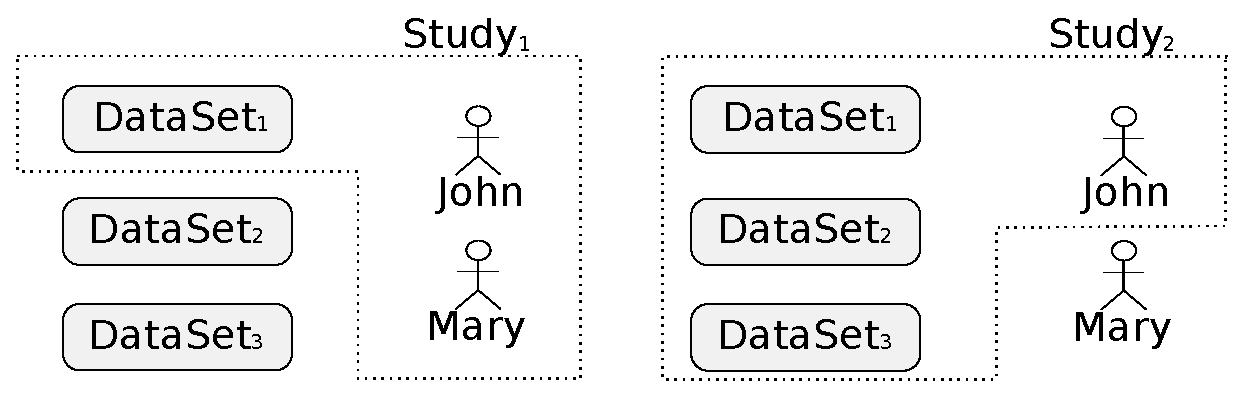
\includegraphics[scale=0.4]{./imgs/projects-as-groupings1.eps}
 % projects-as-groupings1.eps: 0x0 pixel, 300dpi, 0.00x0.00 cm, bb=0 207 582 382.
\caption{Study1 has John and Mary as users and includes DataSet1, while Study2 has only John as as a user and includes DataSet1, DataSet2, and DataSet3.}
\label{fig:studies}
\end{figure}
\vspace{-5mm}
